\section{Tema 4: Krystallografi og resiprokt rom}
\label{tema4}

\begin{table}[!htb]
    \centering
    \caption{Samtale punkter tema 4}
    \begin{tabular}{|c|c|c|r|}
      \hline
      1 & Faste stoff \& Krystaller, basis og gitter &  \autoref{sec:tema4_1} & \cellcolor{green}\quad\quad \\
      \hline 
      2 & Enhetsseller & \autoref{sec:tema4_3} & \cellcolor{green} \\
      \hline
      3 & Wigner-seitz celle & \autoref{sec:tema4_7} & \cellcolor{green} \\
      \hline 
      4 & Kubiske gitter (fcc, bcc, sc) & \autoref{sec:tema4_5} & \cellcolor{green} \\
      \hline
      5 & Miller indekser & \autoref{sec:tema4_6} & \cellcolor{green} \\ 
      \hline
      6 & Reelt og Resiprokt rom/gitter & \autoref{sec:tema4_8} & \cellcolor{blue} \\
      \hline
    \end{tabular}
    \label{tab:samtalePunkt_tema1}
\end{table}

\subsection{Faste stoff \& Krystaller, basis og gitter}
\label{sec:tema4_1}
Faser er en måte å beskrive tilstanden til stoffer, vi har gass, væske og fast form. Vi ser på faste stoffer, dermed er det mest interessant å se på fast form. Fast form kan deles inn i ordnet og uordnet, der ordnet betyr regelmessig arrangement av atom (langt-rekkende ordning) eller krystallinsk tilstand. For uordnede faste stoffer vil atomene ha en tilfeldig ordning, som er en kortrekkende ordning. 

\begin{definition}
    \textbf{Langt-rekkende}. Ved å se hvordan utformingen til et stoff er i (relativt) kort rekkevide, kan man vite hvordan det ser ut langt unna.
\end{definition}

\begin{figure}[!htb]
    \centering
    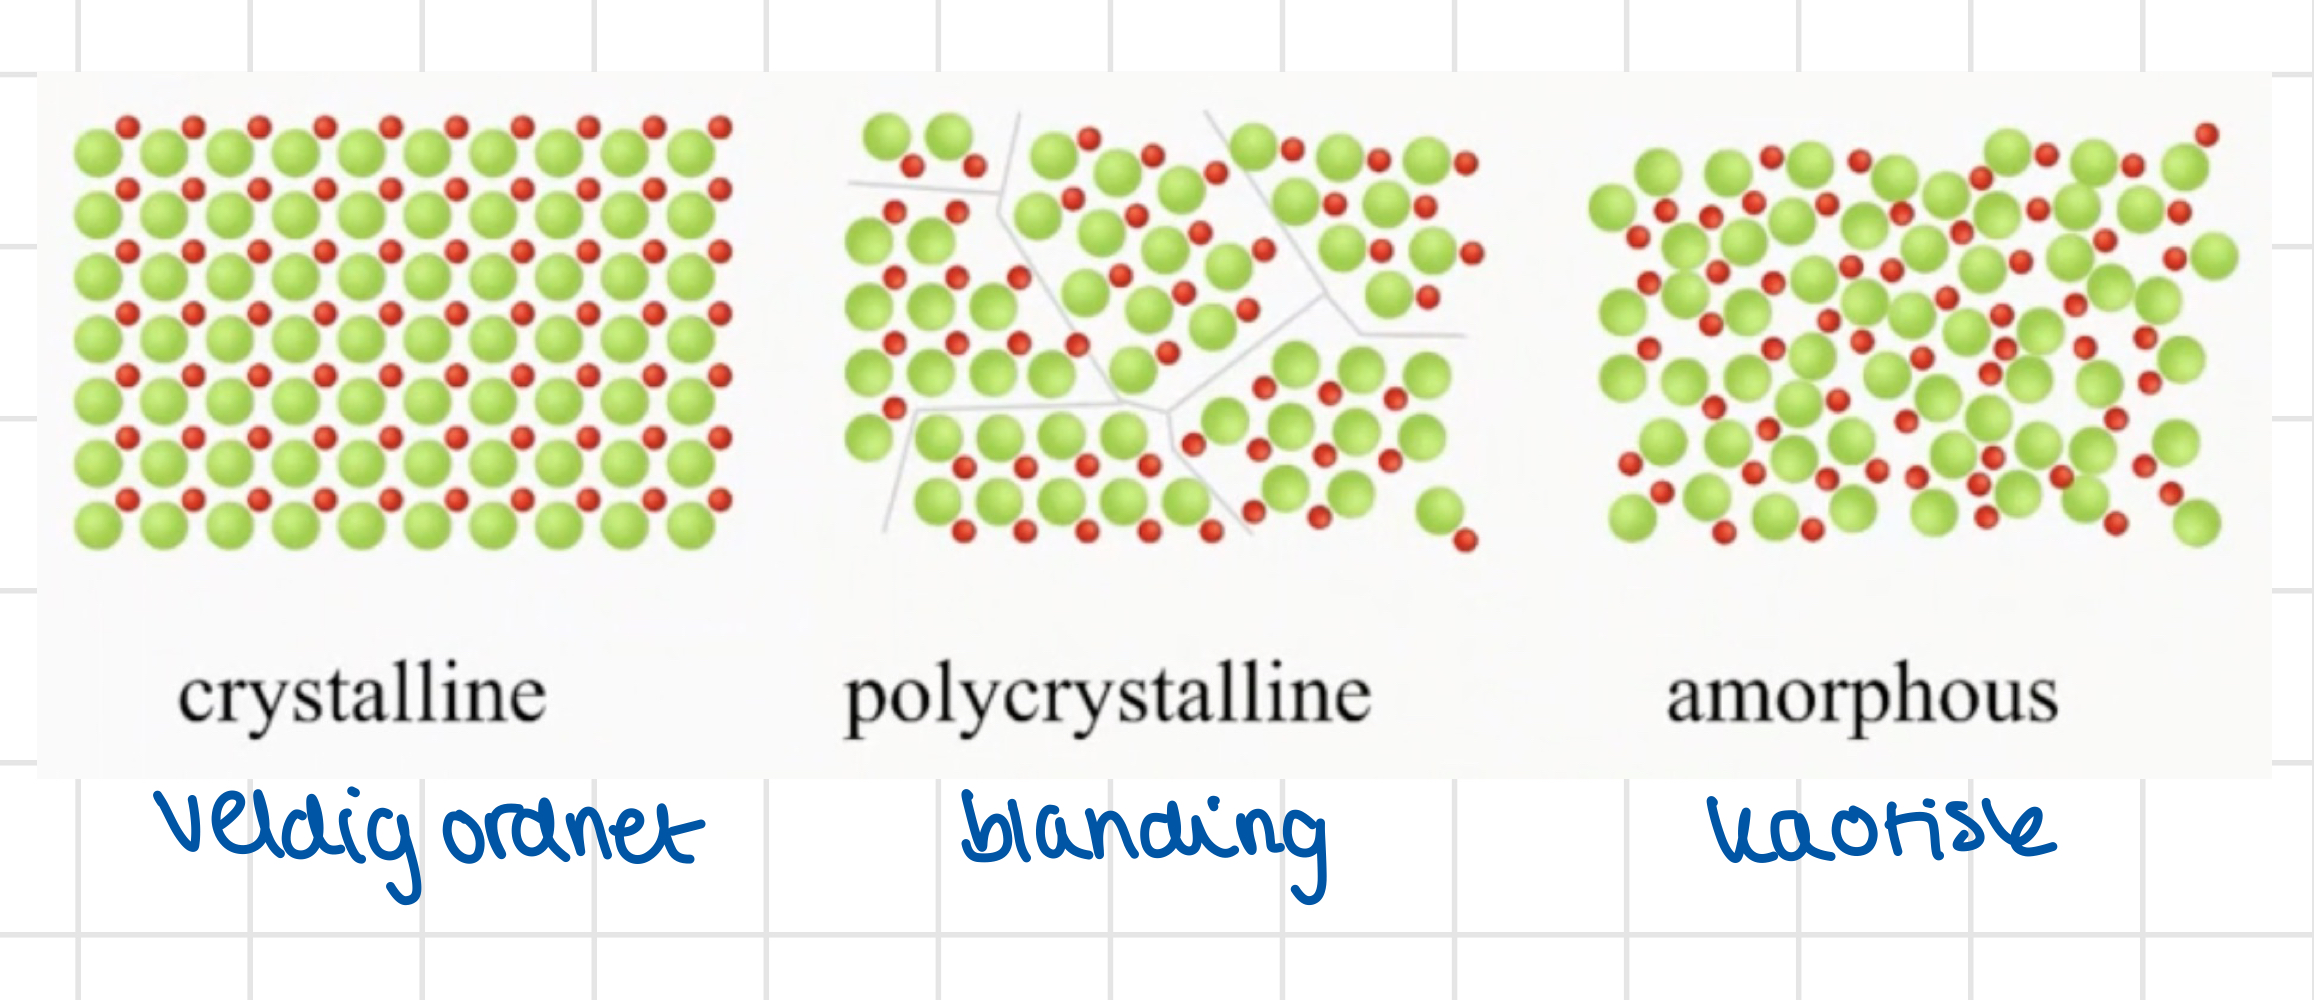
\includegraphics[scale=0.2]{Bilder/SamtaleTema4/Faste Stoffer/faserr.jpeg}
    \caption{Krystallinsk tilstand er veldig ordnet, mens polykrystallinsk delvis ordnet, men amorft er helt kaotisk}
    \label{fig:EskempelOppbygning}
\end{figure}

For å kunne forklare hvordan et stoff er bygget opp kan det være nyttig å innføre den anvendte terminologien. En krystall er satt sammen av en basis og et gitter. \autoref{fig:cryst} viser at basis pluss gitter gir ut krystall. Et gitter er kun et samling matematiske punkt i rommet for å hjelpe oss med å beskrive et stoff. Basisen brukes til å fortelle om sammensetning av atomer som festes til hvert gitterpunkt.

\begin{figure}[!htb]
    \centering
    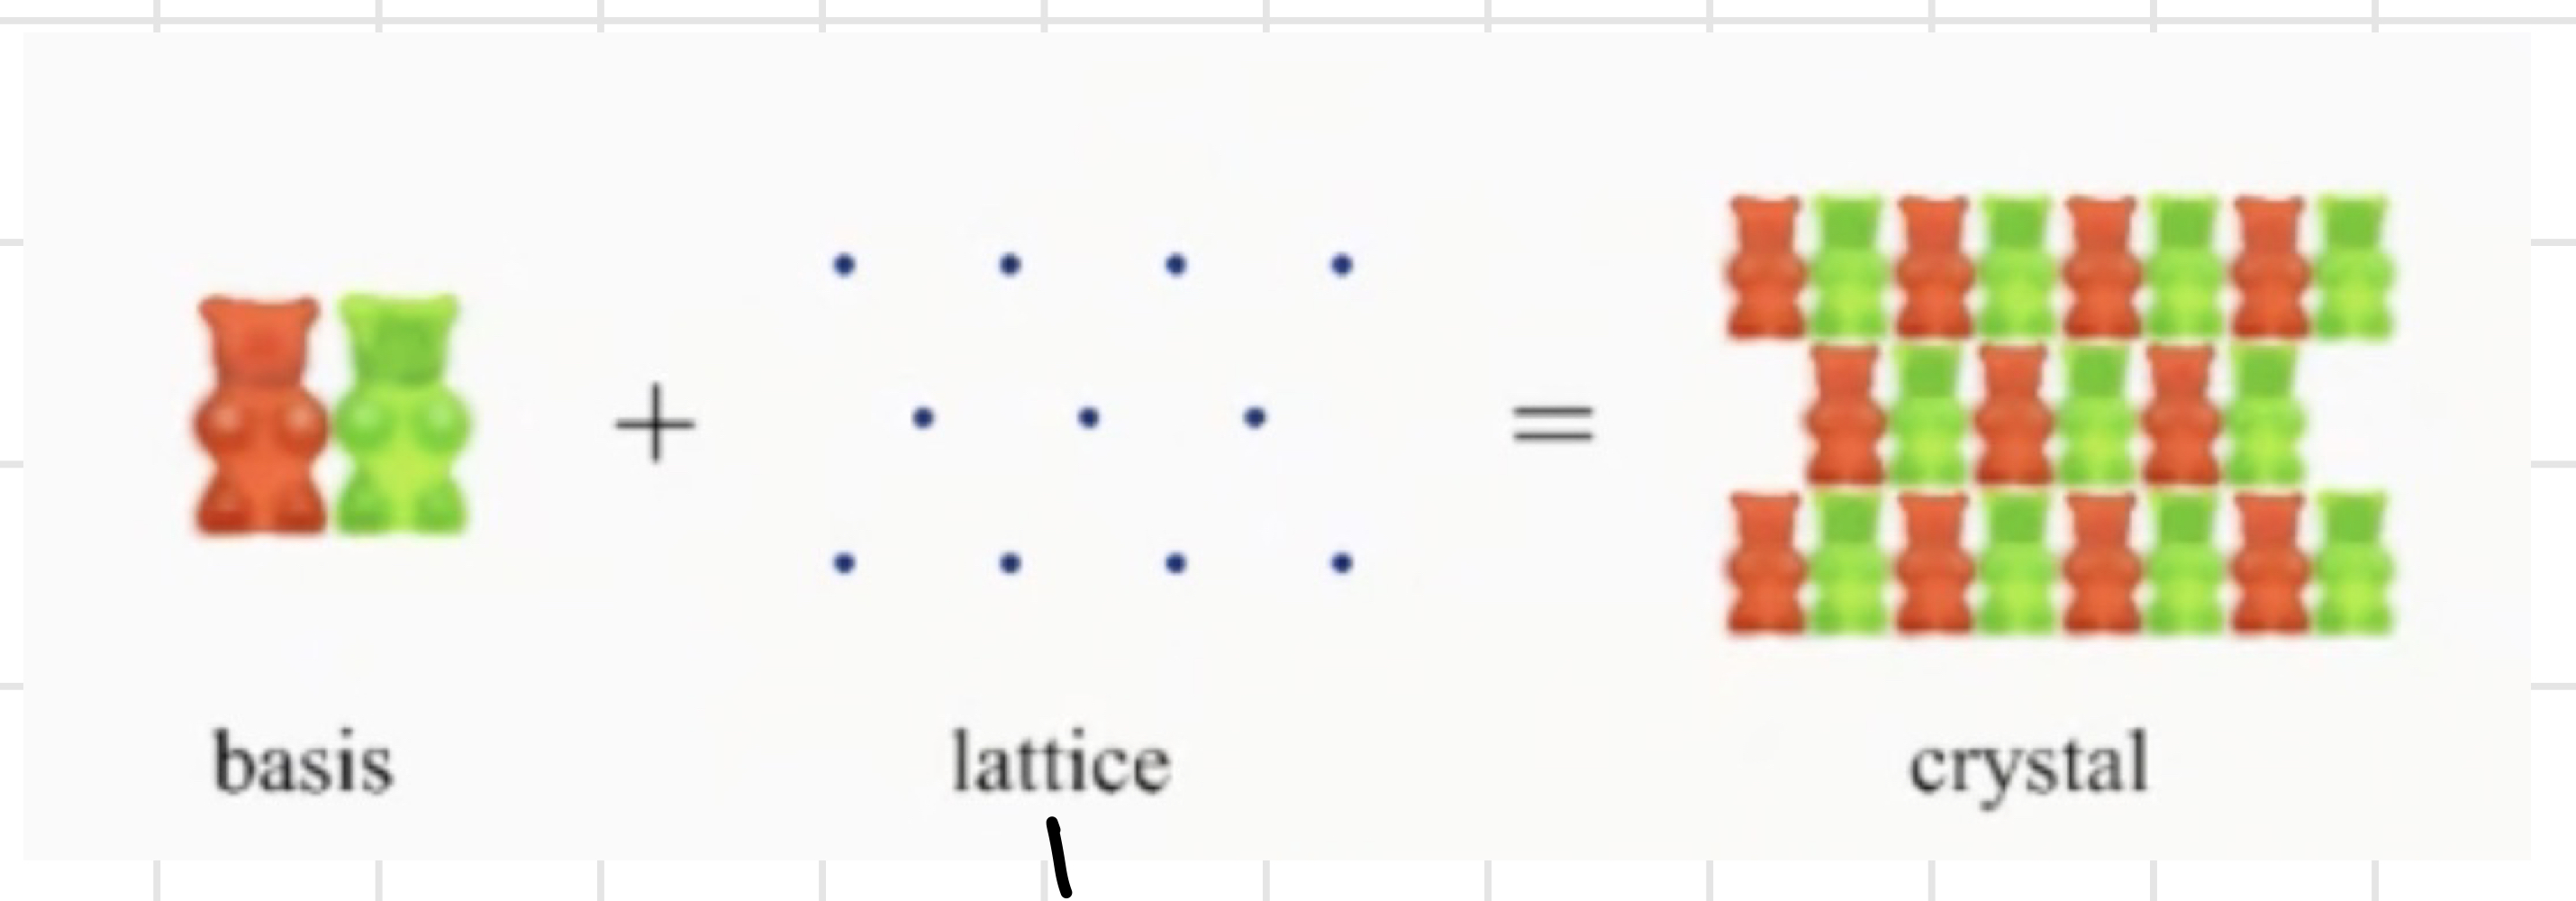
\includegraphics[scale=0.15]{Bilder/SamtaleTema4/Faste Stoffer/krystallKlosser.jpeg}
    \caption{Krystaller er satt sammen av en basis som legges på hvert gitterpunkt (latticepoint)}
    \label{fig:cryst}
\end{figure}

\begin{definition}
    \textbf{Enhetscelle}: er den minste byggeklossen som beskriver gitteret.
\end{definition}

\subsection{Enhetsseller}
\label{sec:tema4_3}
Et gitter kan representeres matematisk i reelt rom,

\begin{equation}
\label{eq:real}
    \Vec{R} = \sum_{i=1}^3 n_i\Vec{a_i},
\end{equation}

Her er $n_i$ positive eller negative heltall som skalerer vektorene $a_i$ i rommet, disse kan også være null. $a_i$ er enhetsvektorene som beskriver gitteret.

\begin{definition}
    \textbf{Bravaisgitter}: 3-dimensjonal konfigurasjon som atomer kan bli arrangert innenfoor krystaller.
\end{definition}

Det finnes 14 typer bravaisgitter som beskriver enhver krystall. \MYhref{https://en.wikipedia.org/wiki/Bravais_lattice}{Wikipedia} viser alle 14 for tre dimensjonelt rom, og 5 for to dimensjonelt.

\begin{definition}
    \textbf{Enhetscellen}: Den minste byggeklossen som beskriver et gitter. Enhetscellen kan ikke ha \textit{ikke periodiske} former.
\end{definition}

Vi kan dele enhetsceller inn i to kategorier, primitive og konvensjonelle. Primitive enhetsceller inneholdeer bare ett gitterpunkt. Konvensjonelle enhetsceller er vanlige konfigurasjoner og kan inneholde mer enn ett gitterpunkt. Det er oftere enklere å finne konvensjonelle enhetsceller. Men vi skal nå se på en systematisk måte å produsere en enhetscelle.

\subsection{Wigner-seitz celle}
\label{sec:tema4_7}
Wigner-Seitz cellen er en bestemt måte å finne en primitiv enhetscelle på. WS-cellen produseres ved å konstruere vektorer fra et gitt gitterpunkt til ''alle andre'' gitterpunkt, for deretter å konstruere linjer (2D) eller plan (3D) på midtpunktet av vektorene.

Kanten av en WS-celle ligger alltid halveis mellom to rekker med atomer. 

\begin{figure}[!htb]
    \centering
    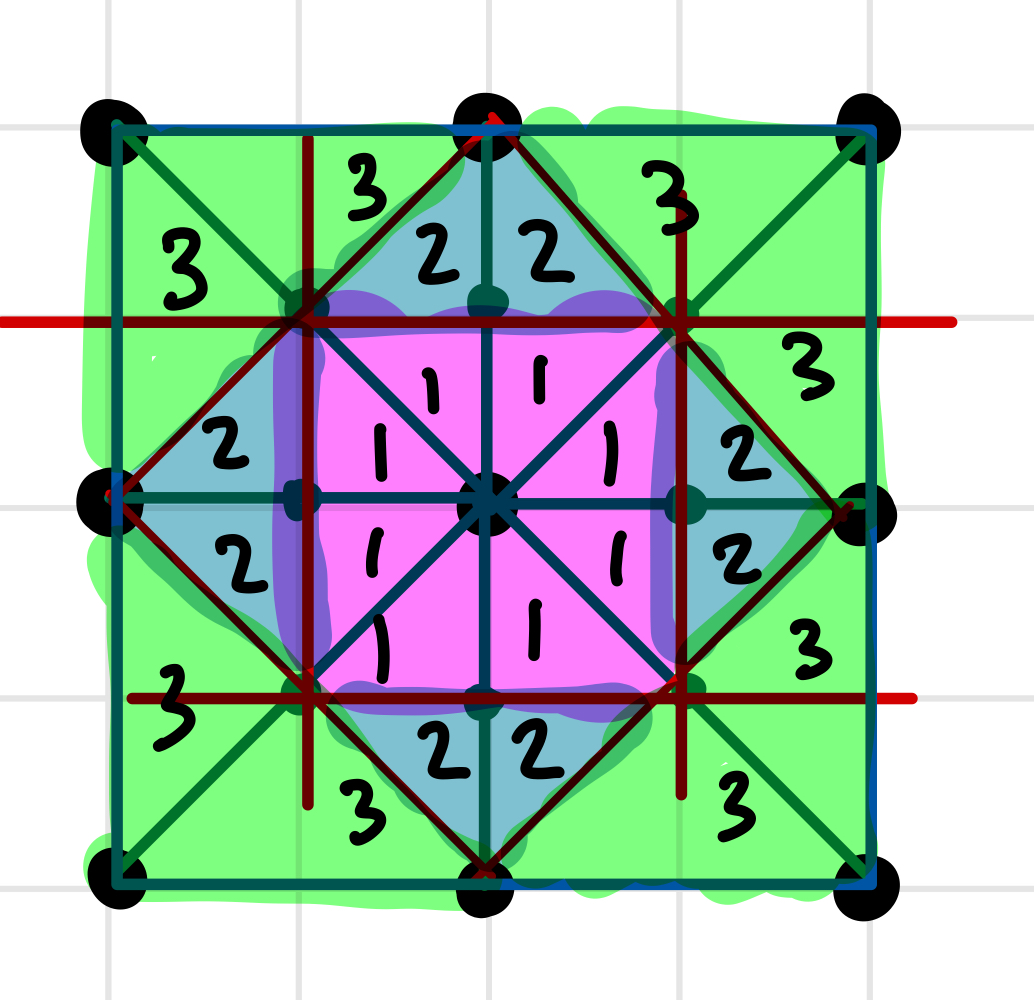
\includegraphics[scale=0.2]{Bilder/SamtaleTema4/WS_Celle.jpeg}
    \caption{Wigner-Seitz cellen, første orden i \color{purple}lilla\color{black}, andre orden \color{blue}{blå} \color{black} og tredje orden i \color{green}{grønn}\color{black}.}
    \label{fig:enter-label}
\end{figure}

\subsection{Kubiske gitter (sc, fcc, bcc)}
\label{sec:tema4_5}
Gitterpunktene til en simple cubic (sc) enhetscelle kan forklares med en tre dimensjonell tegning. Lengdene på alle sidene er like lange, så orienteringen i rom har ikke noe å si for enhetscellen. Som en vanlig er det tre vektorer som møtes til hvilket som helst punkt på kuben, vinkelen mellom disse vektorene er 90$^\circ$. I en sc enhetscell er det totalt ett atom per enhetscelle, det fordeles slik

\begin{equation*}
    \frac{1}{8}\cdot 8 = 1,
\end{equation*}

$\frac{1}{8}$ kommer av et hvert atom deles med \textbf{syv} nabo sc-enhetsceller. 

\begin{figure}[!htb]
    \centering
    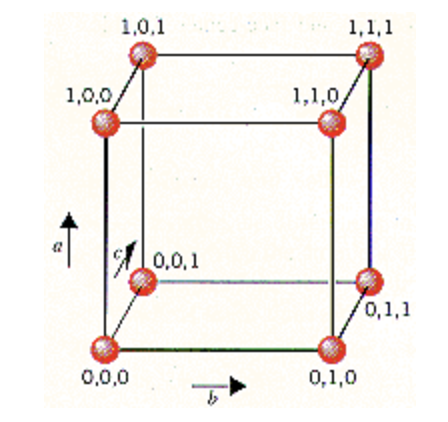
\includegraphics[scale=0.8]{Bilder/SamtaleTema4/sc.png}
    \caption{En simple cubic enhetscelle}
    \label{fig:sc}
\end{figure}
\newpage
Face centered cubic (fcc) er en konfigurasjon mye lik som sc, men i tillegg til hjørnene så er det atomer på hver flate av kuben. Denne enhetscellen har det vi kaller høyest pakketetthet, det vil si at atomene tar opp størst volum av kuben, av de tre enhetscellene vi går inn på. Antall atomer i en fcc er 

\begin{equation*}
    \frac{1}{8} \cdot 8 + \frac{1}{2}\cdot 6 \,= \,4
\end{equation*}

Faktoren på en halv representerer at flatsidene på cellen deles med en identisk celle, dermed får begge ''eierskap'' på halve volumet til atomet og en kube har seks sider.

\begin{figure}[!htb]
    \centering
    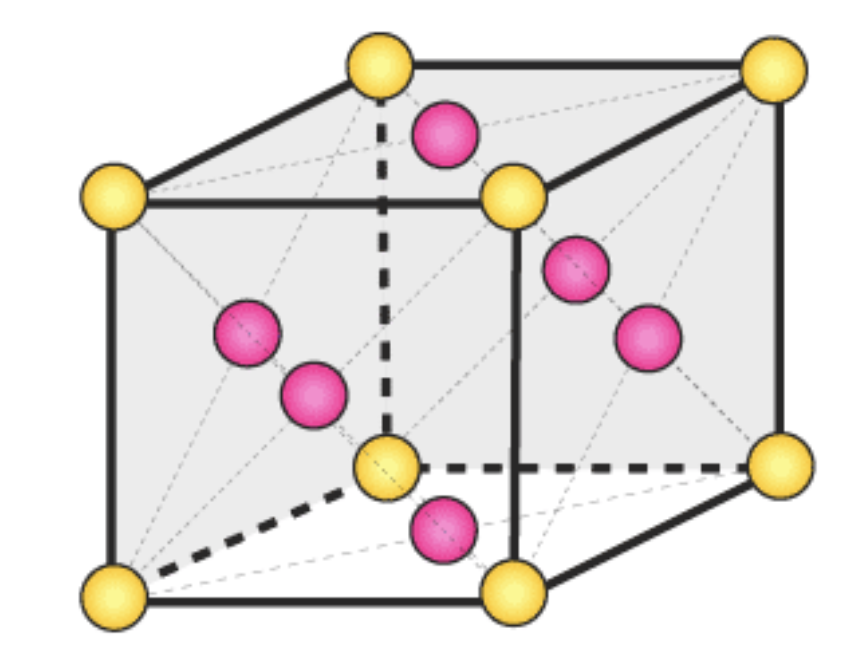
\includegraphics[scale=0.5]{Bilder/SamtaleTema4/fcc.png}
    \caption{Face centered cubic unitcelle.}
    \label{fig:fcc}
\end{figure}

Body centered cubic (bcc) er en enhetscellen akkurat som fcc, som har byggekloss sc i grunn, også finnes det da som navnet tilsier body centered. Et punkt i kjernen av kuben. Dette medfører at totalt antall atomer for en bcc er

\begin{equation*}
    \frac{1}{8}\cdot 8 + 1 = 2
\end{equation*}

\begin{figure}[!htb]
    \centering
    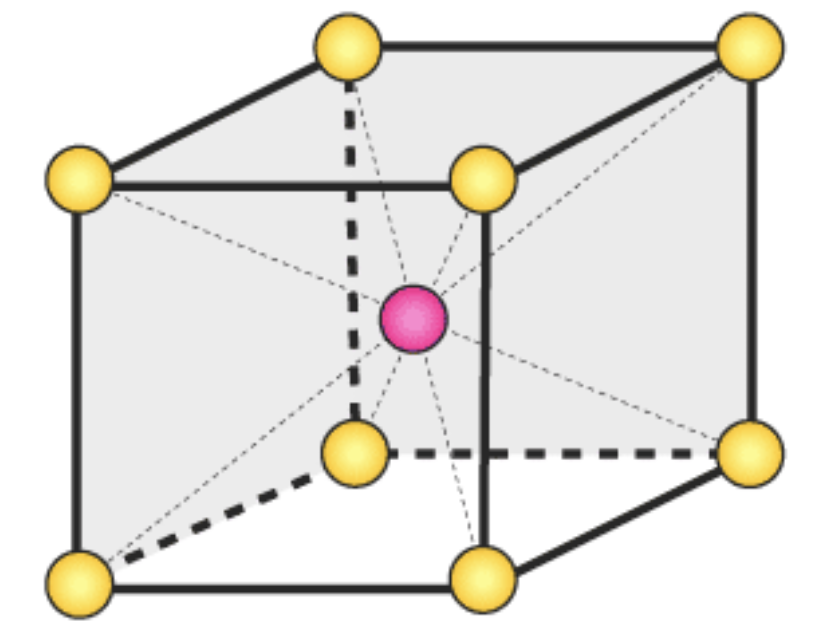
\includegraphics[scale=0.5]{Bilder/SamtaleTema4/bcc.png}
    \caption{Boody centered unit cell}
    \label{fig:bcc}
\end{figure}

\subsection{Miller indekser}
\label{sec:tema4_6}
Miller indekser brukes for å angi retninger i en krystall. Dette er nyttig siden krystaller er an-isotropiske, altså de er ikke like i alle retninger, så avhengig av hvordan du måler de vil krystallen se forskjellig ut og dermed ha forskjellige oppførseler. \autoref{fig:miller} viser alle millerindeksene.

\begin{figure}[!htb]
    \centering
    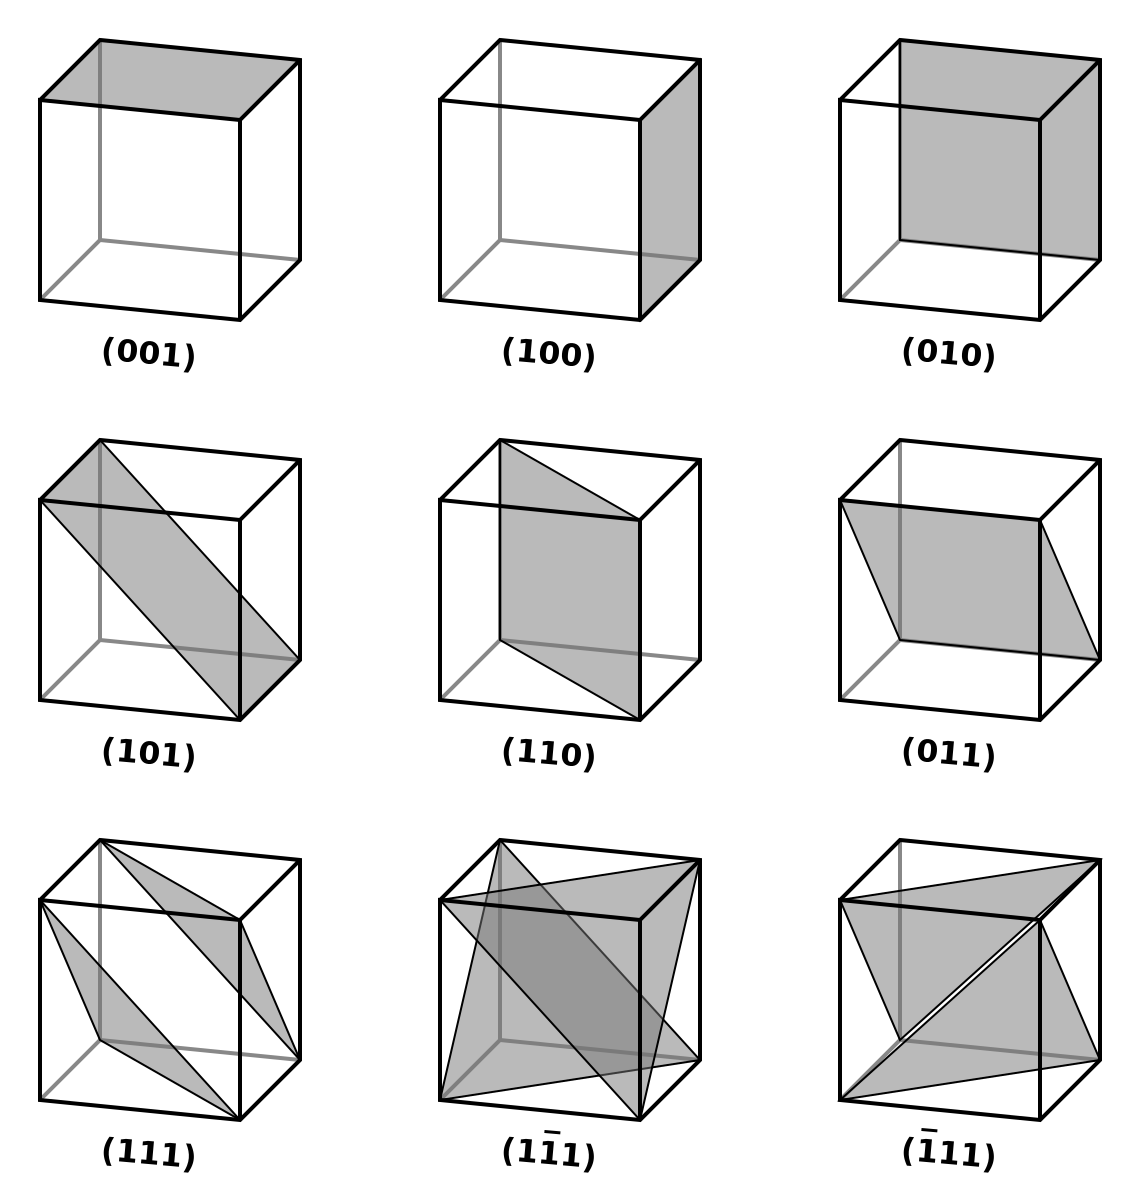
\includegraphics[scale=0.3]{Bilder/SamtaleTema4/miller.png}
    \caption{Alle miller indeksene, bar over tall er en annen notasjon for minus.}
    \label{fig:miller}
\end{figure}

Git et plan, så er det relativt lett å finne Miller indeksen. La oss ta utgangspunkt i indeksen øverst til venstre, $x$ er definert positivt høyre, $y$ inn i arket og $z$ oppover. 

Vi ser at $z$-aksen blir skjært, men $y$- og $x$-aksen går mot uendelig, dermed får vi 

\begin{equation*}
    (\infty \; \infty \; 1) \implies \bigg(\frac{1}{\infty}\;
    \frac{1}{\infty}\; \frac{1}{1}\bigg) = (0\;0\;1)
\end{equation*}
 \newpage
 
\subsection{Reelt og Resiprokt rom/gitter}
\label{sec:tema4_8}
Fourier transformen er mye brukt i signalanalyse, da den gir et forhold mellom et signal og tilhørende frekvenser i signalet. Fourier transformen tar et signal og splitter det i sine respektive komponenter. Mindre verdier i tidsdomenet gir høyere verdier i frekvensdomenet. Dette gjelder også for rom, vi sier derfor at resiprokt rom er Fourier transformen av reelt rom.

\begin{equation}
    \mathscr{F}(\mathbb{R}^n) = \text{Resiprokt rom},
\end{equation}

Vi kan med det si at gitter er romlige frekvenser som Fourier transformeres. I reelt rom har vi i en dimensjon $x$ for avstand, mens i resiprokt rom blir dette $\frac{1}{x}$. I en tre dimensjonell situasjon får vi da frekvenser i flere dimensjoner. Diffraksjon kan benyttes for forståelse av dette. 

\begin{figure}[!htb]
    \centering
    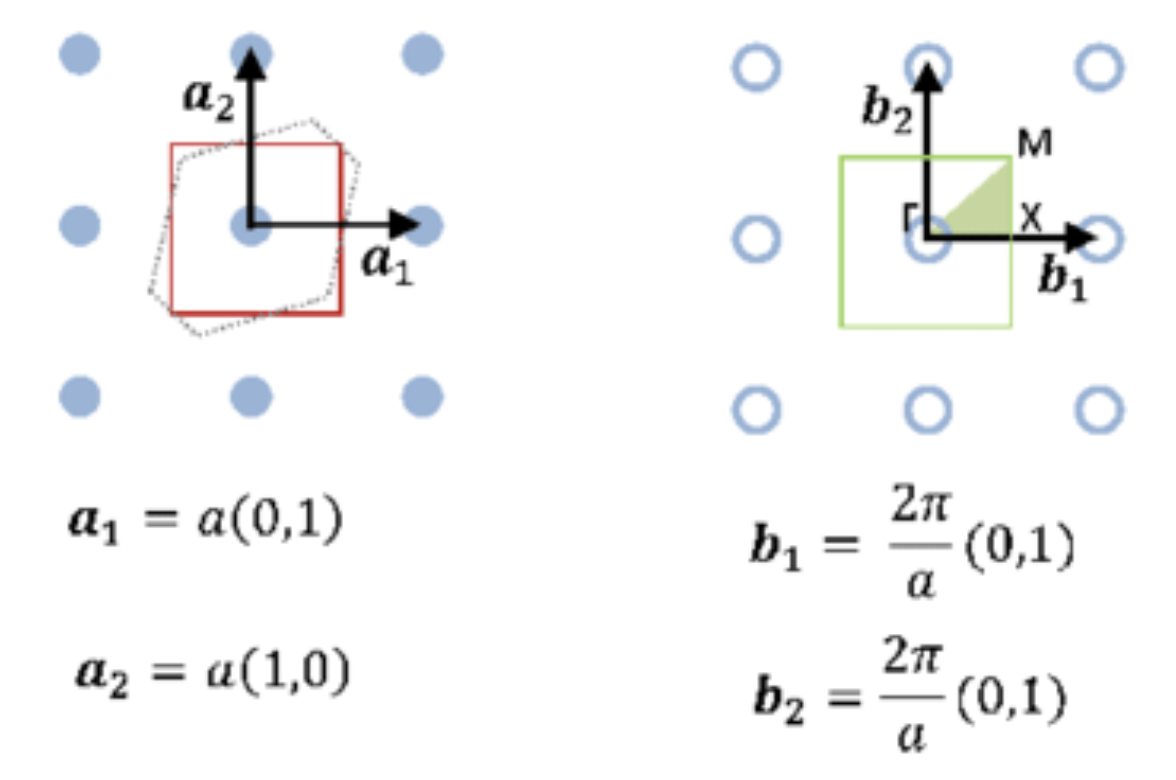
\includegraphics[scale=0.4]{Bilder/SamtaleTema4/resip.png}
    \caption{Overgangen fra reelt rom til resiprokt rom, faktoren $2\pi$ er en konsekvens av Fourier transformen.}
    \label{fig:resip}
\end{figure}

Vi har vært gjennom sc, fcc og bcc. Det skjer noe interesant når vi Fourier transformerer disse.

\begin{equation*}
    \begin{split}
        \textbf{sc} &\xrightarrow{\mathscr{F}} \textbf{sc}\\
        \textbf{fcc} &\xrightarrow{\mathscr{F}} \textbf{bcc}\\
        \textbf{bcc} &\xrightarrow{\mathscr{F}} \textbf{fcc}\\
    \end{split}
\end{equation*}

I motsetning til relle gittervektorer som kan beskrives med ligning \ref{eq:real}, så beskrives resiproke gittervektorer annerledes, blandt annet ved hjelp av MillerIndeksene.

\begin{equation}
    \label{eq:resiprok}
    \Vec{G}_{hkl} = h\Vec{b}_1 + k \Vec{b}_2 + l \Vec{b}_3,
\end{equation}

Eventuelt kan de skrives på formen 
\begin{equation}
\label{eq:resiprok2}
    \Vec{G}_{hkl} = \frac{2\pi \Vec{n}_{hkl}}{d_{hkl}}
\end{equation}

I ligning \ref{eq:resiprok2} er $\Vec{n}_{hkl}$ normalvektoren til Miller planet, og $d_{hkl}$ er den inter-planære avstanden, det vil si avstanden parallelt mellom to plan.

En rotasjon mellom reelle og resiproke basisvektorer kan beskrives med en syklisk permutasjon:

\begin{equation}
\label{eq:syklisk}
    \begin{split}
        \Vec{b}_1 &= \frac{2\pi (\Vec{a}_2 \cross \Vec{a}_3)}{\Vec{a}_1\cdot(\Vec{a}_2 \cross \Vec{a}_3)}\\
         \Vec{b}_2 &= \frac{2\pi (\Vec{a}_1 \cross \Vec{a}_3)}{\Vec{a}_2\cdot(\Vec{a}_1 \cross \Vec{a}_3)}\\
          \Vec{b}_3 &= \frac{2\pi (\Vec{a}_2 \cross \Vec{a}_1)}{\Vec{a}_3\cdot(\Vec{a}_2 \cross \Vec{a}_1)}
    \end{split}
\end{equation}

fra ligning \ref{eq:syklisk} følger det at 

\begin{equation*}
    \Vec{a}_i\cdot\Vec{b}_j = 2\pi\delta_{ij}
\end{equation*}

og 
\begin{equation*}
\begin{split}
    \Vec{G}_{hkl}\cdot \Vec{R}_{n_1n_2n_3} = 2\pi(hn_1&+kn_2+ln_3)\\
    \text{generell vektor i k-rommet}:\\
    \Vec{k} = k_1\Vec{b}_1 + k_2\Vec{b}_2 + k_3\Vec{b}_3
\end{split}
\end{equation*}

Gittervektorene $\Vec{G}$ og $\Vec{R}$ går alltid mellom to gitterpunkt i sine respektive rom, mens $\Vec{k}$ er fri til å gå hvor som helst. Dette er grunnen til at $\Vec{k}$ vil være en resiprok gittervektor når:

\begin{equation}
    \label{eq:kResi}
    e^{i\Vec{k}\cdot\Vec{R}} = e^{i\Vec{G}\cdot\Vec{R}} = 1
\end{equation}



\MYhref{https://www.youtube.com/watch?v=DFFU39A3fPY}{Denne videoen er henter fra forelesning, og gir en visualisering av resiprokt rom.}

Vi skal nå se på diffraksjon igjen, og som for Youngs eksperiment så vi at dersom vi hadde lys i 3D endte dette opp som plan i 2D. Vi tolker diffraksjon som bølgenes evne til å bøye seg rundt hjørner. 

Vi kan se for oss at vi skyter røntgen stråling (x-rays) på et periodisk atomært gitter (1D), vi får da plan/streker. Sender man det på et to dimensjonalt array gir det istedet punkter, dette er fordi vi får diffraksjon i to plan, istedet for ett.

\begin{figure}[!htb]
    \centering
    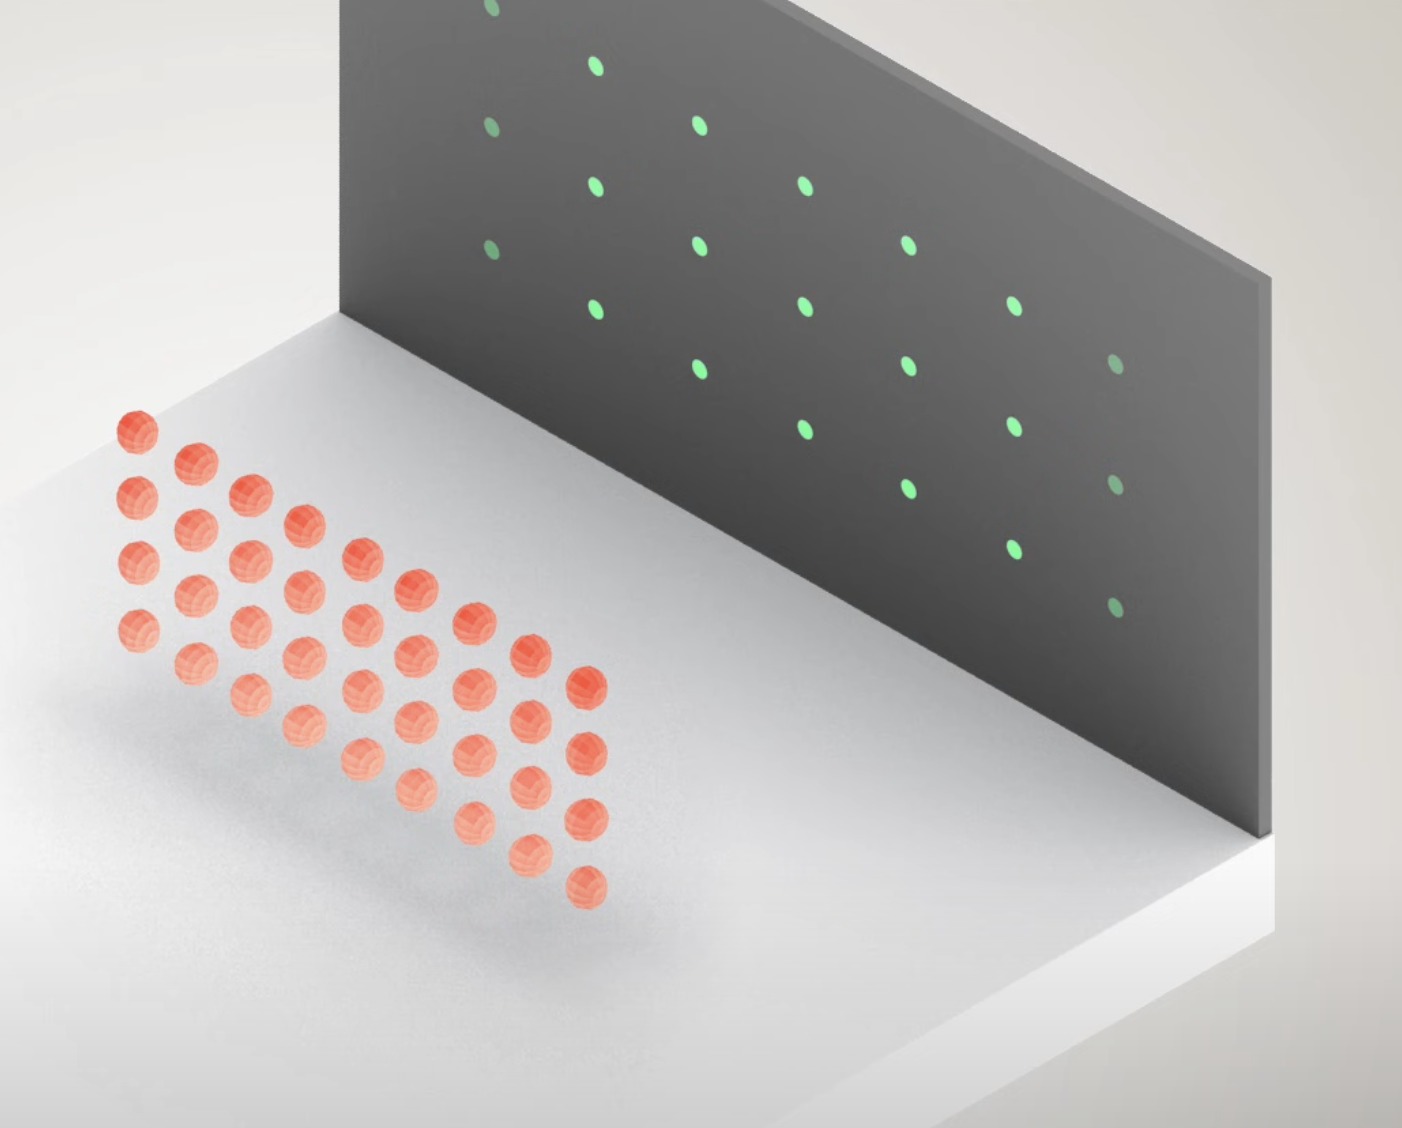
\includegraphics[scale=0.45]{Bilder/SamtaleTema4/2D-array.png}
    \caption{2D-array som produserer interferens i et gitter mønster}
    \label{fig:2d-array}
\end{figure}

\autoref{fig:2d-array} viser et 2D-gitter som får røntgen stråling på seg, på veggen danner det seg et gitter. Dette gitteret ser ut til å ha større avstand mellom punktene enn 2D-gitteret. Det vi ser på veggen er en avbildning av det resiproke rommet! Så dersom avstanden $a$ er mindre enn $1m$ vil avstanden i det resiproke rommet være større, når $a$ øker vil avstanden i reelt rom øke, og avstanden i resiprokt rom minke, husk at forholdet er invers proporsjonalt.

\begin{figure}[!htb]
    \centering
    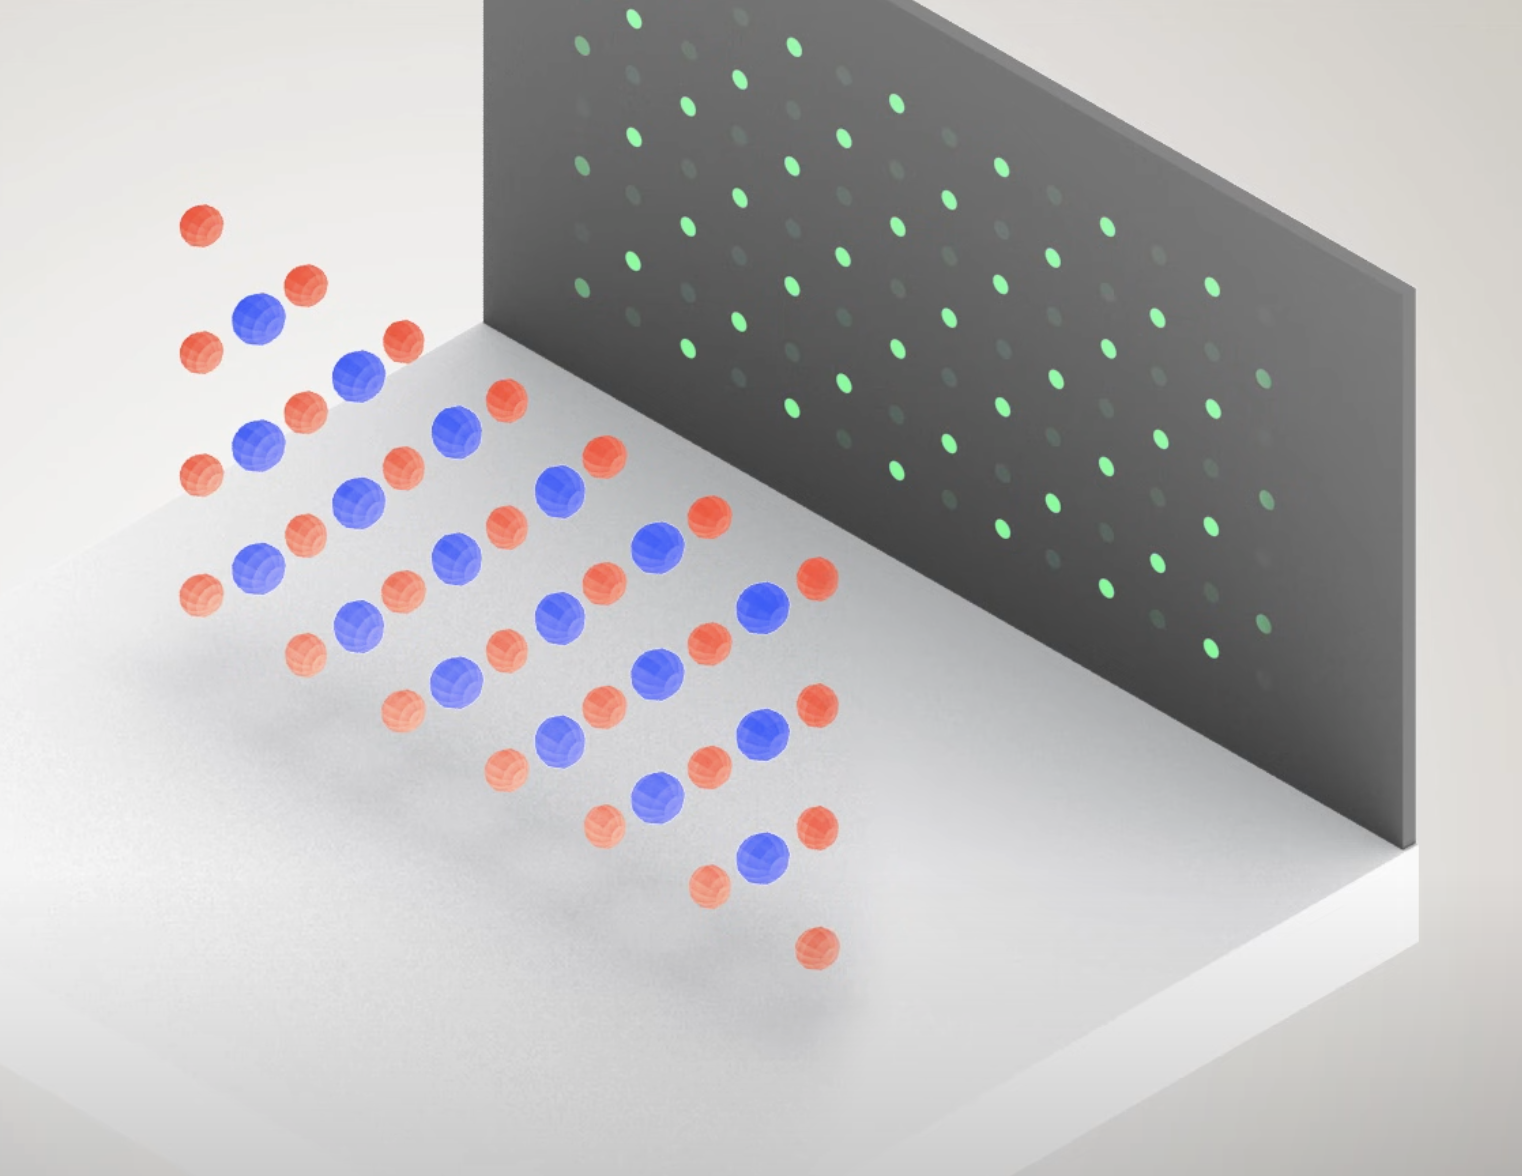
\includegraphics[scale=0.42]{Bilder/SamtaleTema4/skrot.png}
    \caption{Tilegg av atomer mellom gitterpunkt, bevarer periodisitet.}
    \label{fig:periodisity}
\end{figure}

I \autoref{fig:periodisity} er det lagt til atomer mellom gitterpunktene, men uten at de ødelegger krystallens periodisitet. Dette produserer fortsatt de samme interferenspunktene, men det varierer intensiteten.

NB! Som nevnt tidligere er mønsteret som produseres på veggen det gitteret som oppstår i det resiproke rommet. Ved å måle dette kan vi hvordan atomene i faste stoff er organisert.

Resiprokt rom er nyttig for å beskrive hva slags bølger som matcher med en gitt krystall. X-ray-diffraksjon og braggs lov kan brukes for å finne posisjon/avstand mellom atomene:

\begin{figure}[!htb]
    \centering
    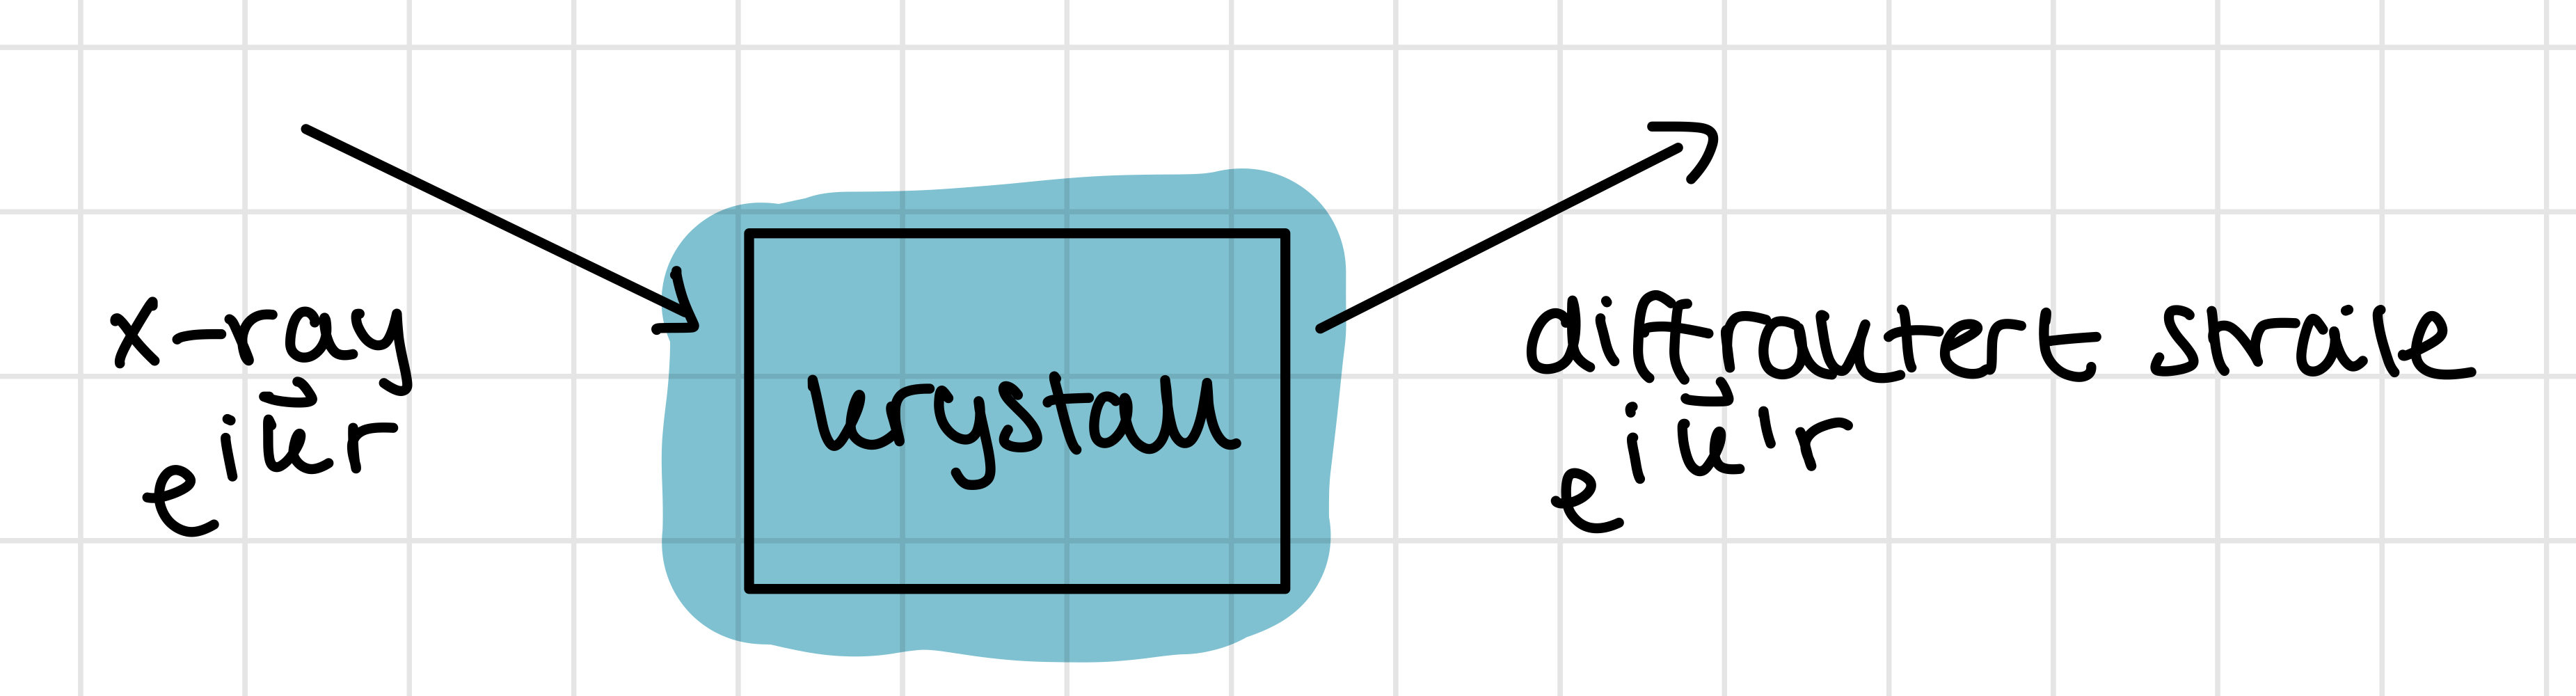
\includegraphics[scale=0.1]{Bilder/SamtaleTema4/diffraksjon.jpeg}
    \caption{Ved å skyte røntgen stråling på en krystall vil man produsere en diffraktert stråle}
    \label{fig:diffrak}
\end{figure}

For å oppnå konstruktiv interferens vil vi trenge at braggs lov er oppfylt, det vil si at ligning \ref{eq:braggs} er oppfylt.

\begin{equation}
\label{eq:braggs}
    2dsin(\theta)= n\lambda
\end{equation}

Det er også betingelser for den diffrakterte strålen, diffraksjon vil kun oppstå når 

\begin{equation}
    \Delta\Vec{k} = \Vec{k'}-\Vec{k} = \Vec{G}
\end{equation}

eller

\begin{equation}
    2\Vec{k}\cdot\Vec{G} = |\Vec{G}|^2
\end{equation}

Brillouisonen er den resiproke versjonen av Wigner-Seits cellen fra reelt rom. Planene vi som dannes mellom to Brillouisoner kalles bragg-plan. Dersom en bølge med riktig bølgelengde treffer dette planet, vil det oppstå konstruktiv interferens.

\newpage

